\documentclass{article}%
\usepackage[T1]{fontenc}%
\usepackage[utf8]{inputenc}%
\usepackage{lmodern}%
\usepackage{textcomp}%
\usepackage{lastpage}%
\usepackage{authblk}%
\usepackage{graphicx}%
%
\title{Sparstolonin B, a Novel Plant Derived Compound, Arrests Cell Cycle and Induces Apoptosis in N{-}Myc Amplified and N{-}Myc Nonamplified Neuroblastoma Cells}%
\author{Emily Jacobs}%
\affil{Department of Biology and Biochemistry and the Centre for Regenerative Medicine, University of Bath, Bath, United Kingdom, \newline%
    Department of Pharmacy and Pharmacology and the Centre for Regenerative Medicine, University of Bath, Bath, United Kingdom}%
\date{01{-}01{-}2013}%
%
\begin{document}%
\normalsize%
\maketitle%
\section{Abstract}%
\label{sec:Abstract}%
You would never know it from the global title, but cancer researchers are on a mission to find out what causes cancer cells to respond so well to their chemotherapy drugs, and how they can learn to tolerate such drugs without harm.\newline%
"They're always sort of following a pattern. Maybe they'll show up from a cancer they've never seen before and they might set up a laboratory to investigate this pattern and their story may change as time passes," said Robyn Dawn Smith, PhD, Esophageal Cancer Foundation.\newline%
Dr. Smith and Michael Wanger, Esophageal Cancer Foundation president, revealed the results of an intensive study into cancer patients' responses to chemotherapy through an article published in the New England Journal of Medicine.\newline%
The findings offered a glimpse into the world of cancer treatment\newline%
"They have been in on this disease for over ten years, and yet people still don't understand that a number of things can cause cancer," explained Smith.\newline%
They include medications that change the lining of the esophagus, such as polysomnium, a bacterium which attacks the food you swallow. Those antibiotics cause inflammation of the esophagus, which can put the person's quality of life at risk.\newline%
Dr. Smith believes it's easy to focus on these tiny things, because it's usually far easier to go off drugs on the side of a tumor, than have to worry about a cancer.\newline%
"It's one thing to acquire them from the operating room, it's another thing to put them down your throat to try to prevent cancer. They're very powerful, very effective," said Smith.\newline%
Professors, surgeons and researchers from Boston University, Washington University School of Medicine, Cancer Research University, and the University of Kentucky teamed up to study the patients of 171 different cancer patients to learn about their effects on cancer treatment.\newline%
Sharon Morrison spent seven years undergoing a grueling and aggressive treatment for colorectal cancer.\newline%
"Nothing he was doing changed the outcome of the disease," said Morrison.\newline%
The survival rate among cancer patients after a battle with esophageal cancer may not compare to that of other major medical procedures, but the oncologists and researchers noted that the rate of the type of cancer patients expressing suppressed esophageal expression was the highest observed in the study.\newline%
"And we also found that this clinical response effect is normal," added Dr. Smith.\newline%
Cancers that show strong esophageal expression are those that undergo chemotherapy. These are the cancer patients in the study that had a cure and responded well to chemotherapy.\newline%
The study, published in July 2012, revealed that patients with suppressed esophageal expression tended to be those that had previously received a promising cancer drug called Cucronate, or currently available drugs called noxocomethylate and and eobaribrix.\newline%
Overall survival for the study was 81\%, and Dr. Smith notes that this will remain to be seen.\newline%
"There are a number of trials that are ongoing that we'll be able to keep in mind as we come forward with additional data, and that's for our patients."\newline%
Results from the study will be used to help identify the best potential treatments for esophageal cancer.\newline%
This research should help to lead to more effective treatments, and potentially better results for some types of cancer patients.

%
\subsection{Image Analysis}%
\label{subsec:ImageAnalysis}%


\begin{figure}[h!]%
\centering%
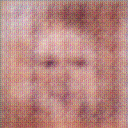
\includegraphics[width=150px]{500_fake_images/samples_5_489.png}%
\caption{A Close Up Of A Baseball Glove On A Field}%
\end{figure}

%
\end{document}